%!TEX root = thesis.tex
\chapter{Tensor Network Theory}
This section begins from a fundamental question: How to draw a tensor network diagrams? In tensor network theory \cite{jordan_studies_2011} \cite{orus_practical_2014} \cite{bauer_tensor_2011}, we are used to represent tensors graphically instead of complicated equations, because \textit{tensor diagrams} can map to quantum states and geometric lattices explicitly. Base on its clear representation, the implementation of  tensor network algorithms become simply. \section{Representation of tensors in tensor Networks}
\label{notations}
In mathematical concept, a tensor is considered as a multi-dimensional array of scalers. The arrangement of the elements in a tensor is dependent to its \textit{indices} and the \textit{rank} of tensor is equivalent to the number of indices. Thus, a rank-0 tensor is a scaler $(T)$, a rank-1 tensor is a vector $(T_{i})$, a rank-2 tensor is a matrix $(T_{ij})$ and so on. 

Graphically, we usually use a node and few bonds to represent a tensor. Some specified examples are shown in figure \ref{fig211}, the number of bond is equal to the rank of tensor, which means that tensors without bonds, with a single bond, with two bonds and with three bonds can map to scalers, vectors, matrices and rank-3 tensor.

\begin{figure}[ht]
	\centering
	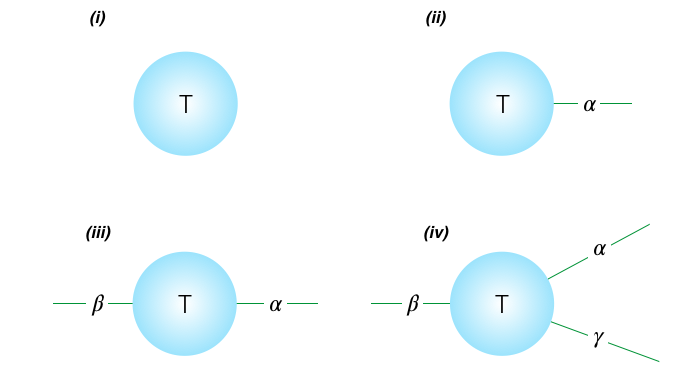
\includegraphics[width=0.75\textwidth]{figures/fig211.png}
	\caption[The reprecentation of commen tensors.]{Usually we use a note and few bonds to compose a tensor and the numbers of bond depend on the rank of tensor. (i) A tensor without bonds is a scaler $T$, (ii) A tensor with one bond is a vector $T_{\alpha}$, (iii) A tensor with two bonds is a Matrix $T_{\alpha \beta}$, (iv) A tensor with three bonds is a rank-3 tensor $T_{\alpha \beta \gamma}$.}
	\label{fig211}
\end{figure}

Then, we should determine the dimension of tensors. Explicitly, the dimension of rank=0 (scaler) is equal to one. However, the dimension of tensors higher than rank-0 depend on the bond dimensions. For instance, in Fig.\ref{fig211}(iv), it's a rank-3 tensor and the dimensions of the indices are $\chi_{\alpha}$, $\chi_{\beta}$, $\chi_{\gamma}$ and T contains $\chi_{\alpha}$$\chi_{\beta}$$\chi_{\gamma}$ components.

\section{Tensor operations and tensor network diagrams} % (fold)
\label{operation}
Basically we can't calculate an fold tensors directly. So the first step, we should unfold tensors. On the other words, we must make their rank lower than 3 before operating. The process is also called \textit{permuteation}.

\subsection{Permutation}
Fig\ref{fig224} is a simple permutation example which means that the tensor $A$ permuted into tensor $\hat{A}$, 
\begin{figure}[ht]
	\centering
	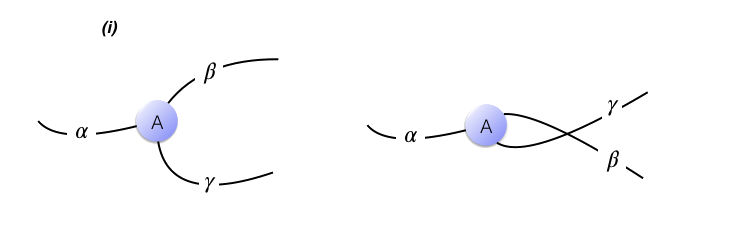
\includegraphics[width=0.75\textwidth]{figures/fig224.png}
	\caption[The process of permuting a tensor.]{Simple example of a tensor permutation. Permute tensor $A$ from indices $\alpha \beta \gamma$ to $\hat{A}_{\alpha \gamma \beta}$ }
	\label{fig224}
\end{figure}
\begin{align}
	A_{\alpha \beta \gamma} \rightarrow \hat{A}_{\alpha \gamma \beta}
\end{align}
The components of $\hat{A}$ and $A$ are equivalence, but having different arrangements.
In order to explaining clearly, I use two flags, incoming (BD\_IN) and outgoing (BD\_OUT) bonds which are also designed for distinguishing different types of \textit{uni10::Bond} in \textit{Uni10}, to show how to reduce the rank of a tensor. Further explanation, BD\_IN and BD\_OUT can be imagined as rows and columns of a matrix. For instance, if the indices of $T_{\alpha \beta \gamma}$ ordered like Fig\ref{fig221}(i), it means that $T_{\alpha \beta \gamma}$ is a matrix $T_{\chi_{\beta}\chi_{\gamma},\chi_{\alpha}}$. Similarity, If it's like Fig\ref{fig221}(ii), it means that $T_{\alpha \beta \gamma}$ is a matrix $T_{\chi_{\beta},\chi_{\alpha}\chi_{\gamma}}$.
\begin{figure}[ht]
	\centering
	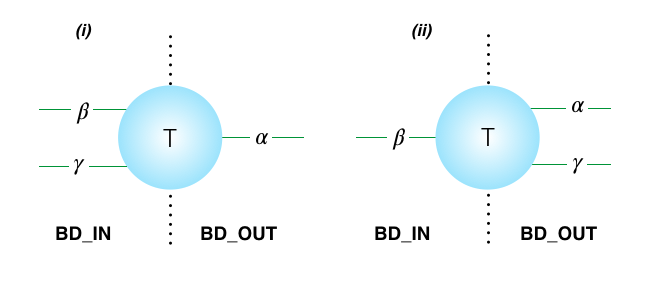
\includegraphics[width=0.75\textwidth]{figures/fig221.png}
	\caption[Representaion of unfold tensors.]{(i) Unfold a tensor to a matrix $T_{\chi_{\beta}\chi_{\gamma},\chi_{\alpha}}$, (ii) Unfold a tensor to a matrix $T_{\chi_{\beta},\chi_{\alpha}\chi_{\gamma}}$.}
	\label{fig221}
\end{figure}
\subsection{Tensor contraction}
Tensor contraction is defined as the sum of all products of the shared indices of tensors. For instance, tensor contraction between two rank-2 tensors $A_{\alpha \beta}$ and $B_{\beta \gamma}$ which is equivalent to inner product between matrix, inner product between matrix $A_{\chi_{\alpha}, \chi{\beta}}$ and $B_{\chi_{\beta}, \chi_{\gamma}}$
\begin{align}
	C_{\alpha \gamma}=\sum\limits_{\beta = 1}^{\chi_{\beta}}{A_{\alpha \beta}B_{\beta \gamma}},
\end{align}
and the tensor diagram is shown in Fig\ref{fig222}(i),
\begin{figure}[ht]
	\centering
	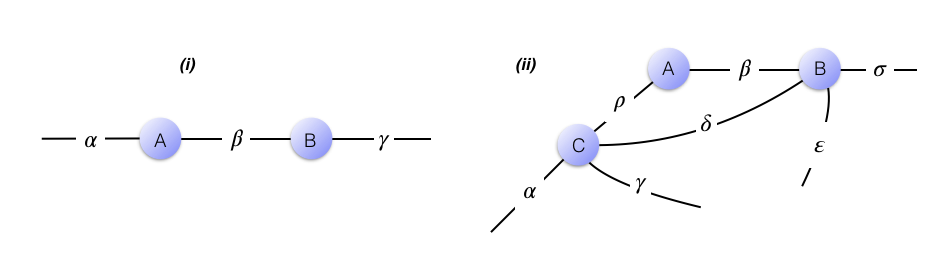
\includegraphics[width=0.75\textwidth]{figures/fig222.png}
	\caption[Simple examples of tensor diagrams.]{(i) Contraction between $A_{\alpha \beta}$ and $B_{\beta \gamma}$ is equivalent to inner product between matrix $A_{\chi_{\alpha}, \chi{\beta}}$ and $B_{\chi_{\beta}, \chi_{\gamma}}$ (ii) A simple tensor network}
	\label{fig222}
\end{figure}

Now we considered a more complexity network, in Fig\ref{fig222}(ii). The equations is written as, 
\begin{align}
	D_{\alpha \gamma \sigma \epsilon}=\sum_{\beta \rho \delta}{A_{\rho \beta}B_{\beta \sigma \epsilon \delta}C_{\gamma \delta \rho \alpha}},
\end{align}
The contraction processes of this network can be separated to some steps.
\begin{figure}[ht]
	\centering
	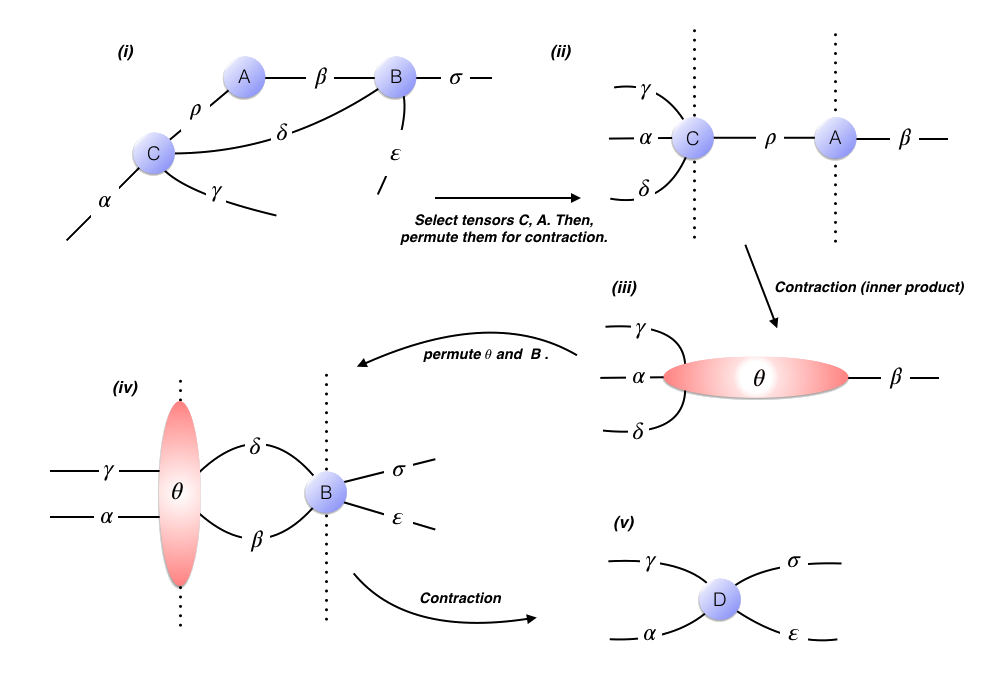
\includegraphics[width=0.75\textwidth]{figures/fig223.png}
	\caption[The contraction processes of the example network which shown in Fig\ref{fig222}(ii)]{ The contraction processes of the example shown in Fig\ref{fig222}}
	\label{fig223}
\end{figure}

(i) First, select a pair of tensors arbitrarily. In Fig\ref{fig223}, we chose beginning from contracting tensors A and C . Actually, this step is very crucial. For example, If the dimensions of each bonds are the same and we select tensor B and C instead, it not only enlarge computational consumption, but also make algorithms inefficient. I'll discuss more detail in \ref{optctm}.(ii) Second, $A$ and $C$ should permute into legal shape. In this case,  $A$ and $C$ are permuted into $A_{\gamma \alpha \delta \rho}$ with one BD\_OUT and $C_{\rho \beta}$ with one BD\_IN, therefore the question evolves to inner product matrix $A_{\chi_{\gamma}\chi_{\alpha}\chi_{\delta}, \chi_{\rho}}$ and $A_{\chi_{\rho}, \chi_{\beta}}$.Repeated step (i) and (ii) again, after getting the tensor $\theta_{\gamma \alpha \delta \beta}$. Permute tensors $\theta$ and $B$ into $\theta_{\gamma \alpha \delta \beta}$ having two BD\_OUT and $B_{\delta \beta \sigma \epsilon}$ having two BD\_IN and we will get tensor $D$, after contracting them by matrix multiplication.

\section{Describe Quantum states with tensor network} % (fold)
\label{sub:map2quan}
Before drawing a many-body system with TN, we should discuss how to describe a chain of N particles, with each particle having $d$ different states and why using TN. Hence, we considered a many-body systems is composed of many local particles and have studied that a pure state corresponds to a vector in Hilbert space, so we intuitively imagined that the wave-function of systems can be written as,
\begin{align}
	\Ket{\Psi_{N}} =\sum_{i_1,i_2,\ldots,i_N}{C_{i_1,i_2,i_3,\ldots,i_N}\Ket{i_1}\otimes\Ket{i_2}\otimes \ldots \otimes \Ket{i_N}},
	\label{wavefunc}
\end{align}
each individual $\Ket{i_1}, \Ket{i_2},\ldots, \Ket{i_N}$ spanned by an orthogonal basis which the degree of freedom is $d$. After writing down the eq.\ref{wavefunc}, we are able to build a TN for quantum states,
\begin{figure}[ht]
	\centering
	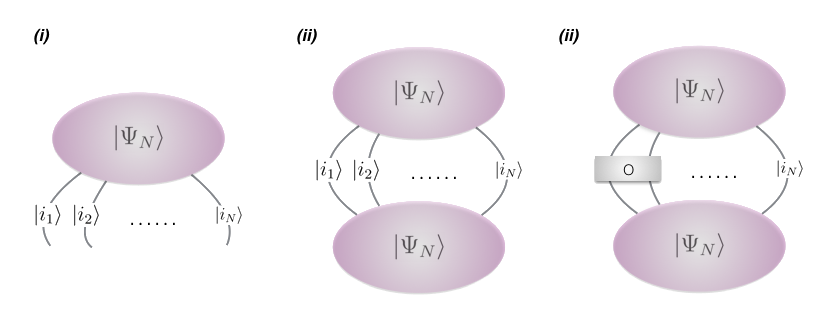
\includegraphics[width=0.75\textwidth]{figures/fig225.png}
	\caption[Represent wave-function of quntum states of TN]{(i) Wave-function: $\Ket{\Psi_N}$ (ii) Norm of $\Ket{\Psi_N}$; $\Braket{\Psi_N|\Psi_N}$ (iii) Expectation value of observable $O$; $\Bra{\Psi_N}O\Ket{\Psi_N}$}
	\label{fig225}
\end{figure}
each bond of tensor corresponds to the local Hilbert space and the dimensions of each bond is equivalent to the states of particle on $i$ site. The geometric notation of $\Ket{\Psi}$ and some fundamental operations are shown in Fig.\ref{fig225}. 

From \ref{wavefunc}, we are aware of the number of coefficients, $C_{i_1,i_2,i_3,\ldots,\i_N}$, is proportional to $d^N$ and fully describing a many-body system which is too expensive. Fortunately, the wave-function can be decomposed to two subsystem by Schmidt Decomposition and there are more details in chapter.\ref{chapter:2ditebd}. 



